
\documentclass[a4paper,11pt,table]{article}

\usepackage[a4paper,margin=1.25in,footskip=0.25in]{geometry}
\usepackage{amssymb,amsmath,latexsym,color,amsthm,authblk,mathpazo,palatino,bbding,setspace,datetime,breakcites,hyphenat,microtype,diagbox,tikz,xcolor,tkz-graph,subcaption,graphicx,titlesec,amsbsy, listings}
\usepackage{titlesec}
\usepackage{mathptmx}
%\usepackage{times}
%\usepackage{cite}
\usepackage[round,authoryear]{natbib}
\citestyle{authordate}
\usepackage{hyperref,theoremref}
\usepackage[titletoc,title]{appendix}
%\usepackage[author={Souvik Roy}]{pdfcomment}
%\usepackage{parskip}
\usepackage[shortlabels]{enumitem}
\usepackage{float}
\usepackage{amssymb}
\restylefloat{table}
\everymath{\displaystyle}
\usepackage{pstricks}

\usepackage{tikz}
\usetikzlibrary{arrows}




%\usepackage{accents}
%\setlength{\parindent}{15pt}
\usepackage{accents}

\newcommand{\ut}[1]{\underaccent{\tilde}{#1}}
\renewcommand{\vec}[1]{\ut{#1}}

\definecolor{armygreen}{rgb}{0.29, 0.8, 0.13}
\definecolor{auburn}{rgb}{0.43, 0.21, 0.1}
\definecolor{burgundy}{rgb}{0.5, 0.0, 0.13}
\definecolor{medium red}{rgb}{.490,.298,.337}
\definecolor{dark red}{rgb}{.235,.141,.161}

\hypersetup{
	colorlinks = true,
	linkcolor = {burgundy},
	citecolor = {burgundy}, 		
	linkbordercolor = {white},
}

\captionsetup[sub]{font=scriptsize}

% \interfootnotelinepenalty=10000
% \raggedbottom

% \let\OLDthebibliography\thebibliography
% \renewcommand\thebibliography[1]{
% 	\OLDthebibliography{#1}
% 	\setlength{\parskip}{0pt}
% 	\setlength{\itemsep}{0pt plus 0.1ex}
% }

% \DeclareFontFamily{U}{mathx}{\hyphenchar\font45}
% \DeclareFontShape{U}{mathx}{m}{n}{<-> mathx10}{}
% \DeclareSymbolFont{mathx}{U}{mathx}{m}{n}
% \DeclareMathAccent{\widebar}{0}{mathx}{"73}


% Page length commands go here in the preamble
%\setlength{\oddsidemargin}{-0.25in} % Left margin of 1 in + 0 in = 1 in
%\setlength{\textwidth}{7in}   % Right margin of 8.5 in - 1 in - 6.5 in = 1 in
%\setlength{\topmargin}{-.75in}  % Top margin of 2 in -0.75 in = 1 in
%\setlength{\textheight}{9.5in}  % Lower margin of 11 in - 9 in - 1 in = 1 in

\interfootnotelinepenalty=10000
\raggedbottom

\let\OLDthebibliography\thebibliography
\renewcommand\thebibliography[1]{
	\OLDthebibliography{#1}
	\setlength{\parskip}{0pt}
	\setlength{\itemsep}{0pt plus 0.1ex}
}

\newcommand{\va}{\vartriangleleft}
\newcommand{\vaq}{\trianglelefteq}
\newcommand{\rva}{\vartriangleright}
\newcommand{\rvaq}{\trianglerighteq}


\DeclareFontFamily{U}{mathx}{\hyphenchar\font45}
\DeclareFontShape{U}{mathx}{m}{n}{<-> mathx10}{}
\DeclareSymbolFont{mathx}{U}{mathx}{m}{n}
%\DeclareMathAccent{\widebar}{0}{mathx}{"73}

\titleformat{\section}[block]{\normalfont\scshape\large\filcenter}{\thesection .}{1em}{}
\titleformat{\subsection}{\normalfont\scshape\large}{\thesubsection}{1em}{}
\titleformat{\subsubsection}{\normalfont\scshape\large}{\thesubsubsection}{1em}{}
\titleformat{\paragraph}
{\normalfont\scshape\large}{\theparagraph}{1em}{}
\titlespacing*{\paragraph}
{0pt}{3.25ex plus 1ex minus .2ex}{1.5ex plus .2ex}

% Theorem Styles
\newtheorem{theorem}{Theorem}
\newtheorem{proposition}{Proposition}
\newtheorem{claim}{Claim}
\newtheorem{lemma}{Lemma}
\newtheorem{corollary}{Corollary}
\newtheorem{observation}{Observation}[section]
% Definition Styles
\theoremstyle{definition}
\newtheorem{definition}{Definition}[section]
\newtheorem{example}{Example}[section]
\theoremstyle{remark}
\newtheorem{remark}{\textsc{Remark}}[section]

\renewenvironment{proof}[1][\proofname]{{\bfseries #1: }}{\qed}
\newcommand{\tbf}{\textbf}
\newcommand{\sr}{\textcolor{red}}
\newcommand{\srs}{\textcolor{blue}}
\newcommand{\srsk}{\textcolor{armygreen}}
\newdateformat{monthyeardate}{\monthname[\THEMONTH], \THEYEAR}


%%%%%%%%%%%%%%%%%%%%%%%%%%%Code for bg color of code
\usepackage{xcolor}

\definecolor{codegreen}{rgb}{0,0.6,0}
\definecolor{codegray}{rgb}{0.5,0.5,0.5}
\definecolor{codepurple}{rgb}{0.58,0,0.82}
\definecolor{backcolour}{rgb}{0.95,0.95,0.92}

\lstdefinestyle{mystyle}{
    backgroundcolor=\color{backcolour},   
    commentstyle=\color{codegreen},
    keywordstyle=\color{magenta},
    numberstyle=\tiny\color{codegray},
    stringstyle=\color{codepurple},
    basicstyle=\ttfamily\footnotesize,
    breakatwhitespace=false,         
    breaklines=true,                 
    captionpos=b,                    
    keepspaces=true,                 
    numbers=left,                    
    numbersep=5pt,                  
    showspaces=false,                
    showstringspaces=false,
    showtabs=false,                  
    tabsize=2
}
\lstset{style=mystyle}
%%%%%%%%%%%%%%%%%%%%%%%%%

\titleformat{\section}[block]{\normalfont\scshape\large\filcenter}{\thesection .}{1em}{}
\titleformat{\subsection}{\normalfont\scshape\large}{\thesubsection}{1em}{}
\titleformat{\subsubsection}{\normalfont\scshape\large}{\thesubsubsection}{1em}{}


%\newcounter{claim}
%\newenvironment{claim}[1][]{\refstepcounter{claim}\par\noindent\textbf{Claim~\theclaim. #1} \rmfamily}{\medskip}
\renewcommand{\baselinestretch}{1.5} % 1.5 denotes double spacing. Changing it will change the spacing
\renewcommand{\qedsymbol}{$\blacksquare$}
\setlength{\parindent}{.2in}

\setcounter{secnumdepth}{4}

\date{}

\begin{document}

\tableofcontents
\pagebreak
\centerline{ \textbf{\huge Acknowledgement}}
\vspace{8mm}
I would like to express my heartfelt gratitude to Professor Soumyarup Sadhukhan for their invaluable guidance and support throughout the course of this research project. Their expertise, knowledge, and unwavering commitment to academic excellence have been instrumental in shaping the outcome of this report.

I am extremely grateful to Professor Soumyarup for devoting so much time and energy to reviewing and providing constructive feedback on various phases of this research. Their meticulous attention to detail, insightful suggestions, and insightful comments have substantially improved the calibre and rigour of this work.

I would also like to recognise Professor Soumyarup's generosity in sharing their profound insights and expertise in the field. Their mentoring and intellectual discussions have expanded my comprehension of the topic and inspired me to pursue new lines of inquiry.

Lastly, I would like to thank Professor Soumyarup for their unwavering support and encouragement, which served as a constant source of motivation throughout the duration of this research project. Their confidence in my abilities and willingness to invest their time and knowledge were crucial to my academic achievement.

I am extremely privileged to have had the opportunity to work under Professor Soumyarup's supervision. In addition to shaping my academic trajectory, their mentoring has instilled in me a passion for research and a dedication to excellence. I am extremely appreciative of their contributions to this endeavor and their ongoing commitment to fostering an atmosphere of academic excellence. This report would not have been feasible without their incalculable contributions.

I am also indebted to Professor Debasis Mishra for the project report. His note on Mechanism Design (\cite{mishra2008introduction}) helped me to understand the topic in great detail. Some of the definitions and examples presented in this report are taken from that note. 
\vspace{8mm}
\\
Date: \hfill SHABADPREET SINGH\\
12/07/2023 \hfill \hfill Dept. of Mathematics and Statistics
\clearpage

\begin{abstract}\singlespacing

We consider the both-sided matching framework where one side has to be matched with the other side, and both sides have preferences over the other side. In this setting, there are three widely recognized matching algorithms: Deferred Acceptance, Top-trading cycle, and Serial Dictatorship. In this study, we intend to compare the above matching algorithms based on their expected rank-utility under the uniform distribution on the preference profiles. 

		
	\end{abstract}

%\section{Abstract}
% We consider the matching problem where there are two sides to a market, men and women. Each side possesses preferences for individuals on the other side, and they are paired based on these preferences, referred to as both-sided matching. In this setting, there are three widely recognized matching algorithms: Deferred Acceptance, Top-trading cycle, and Serial Dictatorship. In this study, we intend to compare the above matching algorithms based on their expected rank-utility under a probability distribution on the preference profiles. For a matching algorithm, the rank-utility of an agent at a preference profile is $m$-rank of their assigned partner by the algorithm at that profile. The total rank-utility at a preference profile is determined by summing the individual rank-utilities. Ultimately, the expected rank-utility of an algorithm represents the anticipated value derived from these profile-specific rank-utilities.

%  The general version of this problem is inherently complex in a combinatorial sense. Our primary aim is to solve it by assuming a uniform distribution of preference profiles. Using R, we have formulated hypotheses for n agents . Below, we mention the hypotheses.

% \textbf{Hypothesis 1}: According to total rank-utility, Deferred Acceptance is
%  the best algorithm among Deferred acceptance, TTC, and serial dictatorship.

% \textbf{Hypothesis 2:} If we only consider the Men's Side while calculating
% rank-utility, TTC with women as objects is the best algorithm.
% \\
% We have also formulated a \textbf{lemma} for three men and women case that \textit{If a man is assigned to his $3^{rd}$ preferred women in DA, then he will have the same assignment in TTC.}\\
% We have verified the validity of the lemma by examining a wide range of scenarios, including specific and exceptional cases.


% \pagebreak
\section{Introduction}
The \textit{matching theory} is a subfield in game theory where the goal is to match one side with the other. It can be broadly classified into two parts: (a) One-Sided Matching and (b) Two-Sided Matching. One-sided
matching is popularly known as an \textit{object assignment} problem where one side represents the agents, and the other represents the objects. In this model, agents have preferences over the objects, but the objects do not have any preferences. In two-sided matching, both sides represent agents, and they have preferences over the other side.
\\

Matching is one of the most practically applied game-theoretic branches. It has many applications in real-world scenarios, such as school choice, kidney exchange programs, online advertising auctions, allocating housing units, and many more. It is also used in studying labor markets, where firms are matched with workers, or allocating public resources, where public goods are assigned to citizens. In all these contexts, matching is used to design mechanisms that allocate resources among agents efficiently and fairly.
\\

There are several well-known matching algorithms in the literature. In two-sided matching, one such algorithm is \textbf{TTC}, which works given an initial endowment of the objects. Another important algorithm, in this
context, is the \textbf{Serial Dictatorship} algorithm which assumes an ordering over the agents, and the agents get to pick their favorite object according to that ordering. In two-sided matching, the \textit{Gale-Shapley algorithm} is a well-known solution \textit{concept}, which provides a method for finding stable matching in two-sided matching
problems. A matching is stable if no pair of agents (one from each side) have any incentive to break the matching. The Gale-Sahpley algorithm has been used in various practical applications,such as the National Resident Matching Program for medical residency placements in the United States.
\\

The purpose of this paper is to undertake a thorough comparison of the three most prominent matching algorithms in two-sided matching scenarios, DA, TTC, and SD. By analyzing the advantages and disadvantages of both algorithms, we hope to obtain a better understanding of their performance, stability, and fairness. This analysis will provide researchers, practitioners, and policymakers with a greater comprehension of the trade-offs involved when selecting an algorithm for matching in a given context.


%\pagebreak
\section{Basic Framework}
Let $\pmb{M}=\{M_1,\ldots,M_n\}$ be a set of men and $\pmb{W}=\{W_1,\ldots,W_n\}$ be a set of women where $n\in \mathbb{N}$. Every man $M\in \pmb{M}$ has a strict preference $\succ_M$ over the set of women and every women $W\in \pmb{W}$ has a strict preference $\rva_W$ over the set of men.\footnote{A strict preference over a set $S$ is a complete, reflexive, antisymmetric, and transitive binary relation on $S$.} For a preference $\succ$, by $r_k(\succ)$, we denote the $k^{th}$ ranked alternative in $\succ$, i.e., $r_k(\succ)=W$ iff $|\{X\in \pmb{W}\mid XPW\}|=k$.  For $W_x,W_y\in \pmb{W}$ and $M\in \pmb{M}$, $W_x\succ_MW_y$ means $M$  prefers $W_x$ over $W_y$. Similar notations can be defined for a preference $\rva$ over $\pmb{M}$.   We denote the set of all strict preferences over the set $\pmb{W}$ as $\mathbb{L}(\pmb{W})$ and set of all strict preferences over the set $\pmb{M}$ as $\mathbb{L}(\pmb{M})$. By a preference profile $(\succ, \rva)$, we mean a $2n$-tuple of preferences $(\succ_{M_1},\ldots,\succ_{M_n}, \rva_{W_1},\ldots, \rva_{W_n})$ where $\succ_{M_i}$ is the preference of man $M_i$ and $\rva_{W_j}$ is the preference of woman $W_j$ for $i,j\in \{1,\ldots,n\}$. 

A matching $\mu:\pmb{M}\to \pmb{W}$ is a bijective mapping, i.e., it matches a man with a woman. For a matching $\mu$ and $M\in \pmb{M}$, $\mu(M)$ denotes the women, $M$ is matched with in $\mu$. Similarly, for a women $W\in \pmb{W}$, $\mu^{-1}(W)$ denotes the man, $W$ is matched with in $\mu$. We denote the set of all matchings by $\mathcal{M}$.

Below, we define an important and well-known property of a matching. It's called stability. A matching is stable at a preference profile if there is no pair of a man and a woman who prefer themselves over their partners in the matching. Stability ensures that no pair of a man and a woman has any incentive to break the matching. 
\begin{definition}
    A matching $\mu$ is \textbf{unstable} at a preference profile $(\succ, \rva)$ if there exists $M\in \pmb{M}$ and $W\in \pmb{W}$ such that $W\succ_M\mu(M)$ and $M\rva_W \mu^{-1}(W)$. The pair $(M,W)$ is called a \textbf{blocking pair} of $\mu$ at  $(\succ,\rva)$. A matching $\mu$ is \textbf{stable }at $(\succ,\rva)$ if there is no blocking pair of $\mu$ at  $(\succ,\rva)$.
\end{definition}

For example, consider the following preference profile: \label{preference}
\begin{center}
    \begin{tabular}{c|c|c||c|c|c}
        $\succ_1$ & $\succ_2$ & $\succ_3$ & $\rva_1$ & $\rva_2$ & $\rva_3$\\
        \hline
      $W_3$ & $W_3$ & $W_2$ & $M_3$ & $M_2$ & $M_3$  \\
      $W_2$ & $W_2$ & $W_3$ & $M_2$ & $M_3$ & $M_1$ \\
      $W_1$ & $W_1$ & $W_1$ & $M_1$ & $M_1$ & $M_2$ \\
    \end{tabular}
\end{center}
The matching $(M_1:W_1, M_2:W_3, M_3:W_2)$ will be \textit{unstable} as both $M_1 \& W_3$ will prefer each other over their current match, therefore, forming a \textit{blocking pair}.\\
A \textit{stable matching} for the above preference would be $(M_1:W_1, M_2:W_2, M_3:W_3)$. No \textit{blocking pair} exists.


A \textit{matching function} $f$ is a mapping from $\mathbb{L}(\pmb{W})^n \times \mathbb{L}(\pmb{M})^n \to \mathcal{M}$, i.e., for every preference profile $(\succ,\rva)$, matching function assigns a matching.
A matching function is \textit{stable} if it gives a stable matching at every preference profile. In the following, we define another desirable property of a matching function, called \textit{strategy-proofness}. Strategy-proofness guarantees that no one has any incentive to misreport their true preference. In game-theoretic language, it says that truth telling is a dominant strategy. 

\begin{definition}
    A matching function $f:\mathbb{L}(\pmb{W})^n \times \mathbb{L}(\pmb{M})^n \to \mathcal{M}$ is \textbf{strategy-proof for men} if for all $M_i\in \pmb{M}$, and all $(\succ,\rva)\in \mathbb{L}(\pmb{W})^n \times \mathbb{L}(\pmb{M})^n$, and all $\succ'_{M_i}\in \mathbb{L}(W)$, $$f(\succ, \rva)(M_i)\succ_{M_i}f((\succ'_{M_i},\succ_{-M_i}), \rva)(M_i).$$

    Similarly, we can define \textbf{strategy-proofness for women}. A matching function is \textbf{strategy-proof} if it is strategy-proof for both men and women.
\end{definition}
Consider a scenario where there are an equal number of men and women who need to be paired up for marriage. Each individual ranks the members of the opposite gender based on their preferences. The goal is to create stable marriages where no two individuals prefer each other over their current partners.

The \textit{Deferred Acceptance} algorithm is a strategy-proof mechanism that guarantees a stable matching. It works as follows:
\begin{itemize}
    \item Initially, each man proposes to his most preferred woman.
    \item Each woman collects all her proposals and rejects all but her favorite proposal.
    \item Any rejected man proposes to his next preferred woman who has not rejected him yet.
\item The process continues until every woman is paired with a man.
\end{itemize}
Let's see why this algorithm is strategy-proof. Suppose a man tries to manipulate the algorithm by proposing to a woman he does not truly prefer. This woman, according to his ranking, may not be his top choice, but he thinks she is more likely to accept his proposal. However, since the woman collects all proposals and chooses her favorite, she will still reject him if she prefers someone else.

By proposing truthfully, each participant maximizes their chances of getting matched with their most preferred partner. Deviating from truthful preferences will not lead to a better outcome. Hence, the Deferred Acceptance algorithm is strategy-proof in ensuring a stable and fair matching.\\

A matching at a preference profile is \textit{Pareto optimal} if, for every other matching, there exists atleast one man or woman who gets a strictly better match in the current matching. Mathematically speaking, a matching $\mu$ is Pareto optimal at $(\succ,\rva)$ if for every $\mu' (\neq \mu)$, either there is $M\in \pmb{M}$ with $\mu(M)\neq \mu'(M)$ and $\mu(M)\succ_M\mu'(M)$ or there is $W\in \pmb{W}$ with $\mu^{-1}(W)\neq \mu'^{-1}(W)$ and $\mu^{-1}(W)\rva_W\mu'^{-1}(W)$.  A matching function is \textit{Pareto optimal} if it produces a Pareto optimal matching at every preference profile.

\textbf{Example : }Considering the preference profile \ref{preference}, in this case, one possible Pareto efficient matching could be $(M_1:W_1, M_2:W_2, M_3:W_3)$.

In this matching, no man can be assigned to a woman they prefer more than their current assignment. Similarly, no woman can be assigned a man she prefers more than her current assignment. Thus, there is no alternative matching that would make everyone involved happier, making this matching \textit{Pareto efficient}.

\section{Three Important Matching Algorithms}

\subsection{Deferred Acceptance (DA)}

   The \textbf{Deferred Acceptance (DA)} mechanism, also known as the Gale-Shapley algorithm, is a widely used algorithm in matching theory for solving the stable matching problem. It works as follows:
    \begin{enumerate}
        \item Each agent in one set proposes a tentative match to their most preferred agent in the other set.
        \item Each agent receiving proposals considers all the proposals they have received and tentatively accepts the proposal from their most preferred proposer. They reject all other proposals.
        \item Agents who have been rejected in the previous round repeat the process by proposing to their next preferred agent who has not yet rejected them.
        \item The process continues in multiple rounds, with agents proposing and considering proposals until no more proposals are made or rejected.
        \item Once the process reaches a stable state, where no further proposals or rejections occur, the matchings are finalized. Each agent is matched with the partner they tentatively accepted during the process.
    \end{enumerate}
    The deferred acceptance mechanism guarantees the existence of a stable matching, where there are no pairs of agents who would both prefer to be matched with each other rather than their current partners. It ensures that no agent has an incentive to break their assigned match and form a new pair.

\textbf{Example :} Consider the preference profile at \ref{preference}, applying DA;
$$
\textbf{Step 1}
\begin{cases}
{M_1, M_2} \text{ proposes} W_3 \\
{M_3} \text{ proposes} W_2
\end{cases}
$$
As $M_1 \rva_3 M_2$, $W_3$ rejects $M_2$, and {$M_1, M_3$} gets temporarily matched with {$W_3, W_2$}.

$$\textbf{Step 2 :} M_2 \text{ proposes }W_2(M_3)$$
As $M_2 \rva_2 M_3$, $W_2$ rejects
$M_3$(her initial match) and accept the proposal of $M_2$.

$$\textbf{Step 3 :} M_3 \text{ proposes }W_3(M_1)$$
As $M_3 \rva_3 M_1$, $W_3$ rejects
$M_1$(her initial match) and accept the proposal of $M_3$.

$$\textbf{Step 4 :} M_1 \text{ proposes }W_2(M_2)$$
As $M_2 \rva_2 M_1$, $W_2$ rejects proposal of $M_1$.

$$\textbf{Step 4 :} M_1 \text{ proposes }W_1$$
Having received no other proposal $W_1$ accepts his proposal.

$\therefore$ The final matchings are ($M_1:W_1, M_2:W_2, M_3:W_3$).\\

DA is \textit{strategy-proof} and produces \textit{stable} and \textit{Pareto-efficient} matching over all preferences of men and women, though it may not produce Pareto-optimal matching from one side.



\subsection{Top-trading cycle (TTC)}

  The \textbf{Top Trading Cycle (TTC)} algorithm is a mechanism used to solve the problem of two-sided matching, where agents have preferences over potential matches. It works as follows:
    \begin{enumerate}
        \item The algorithm starts by identifying cycles within the preferences. A cycle occurs when a set of agents can be matched in a way that every agent in the cycle prefers their assigned match to any available unmatched agent outside the cycle.
        \item Within each cycle, agents are allowed to trade their current matches with other agents in the cycle to improve their outcomes. The trades occur simultaneously, meaning all exchanges within the cycle happen at once.
        \item The algorithm continues identifying and resolving cycles until no more cycles can be found.
        \item Once all cycles have been resolved, the matches are finalized, and each agent is assigned to their respective match.
    \end{enumerate}
    A TTC with fixed endowment mechanism is \textit{strategy proof and always produces Pareto-optimal matching from men's side.}

\textbf{Example :} Consider the preference profile at \ref{preference}, applying TTC by constructing a directed graph with 3 nodes, one for each man, and putting a directed edge from node of $M_i$ to node of $M_j$ if the top-ranked object of $M_i$ is endowed to $M_j$.

In each graph, men who are part of the \textit{cycle with blue edges} can trade their endowments.\\

\begin{center}
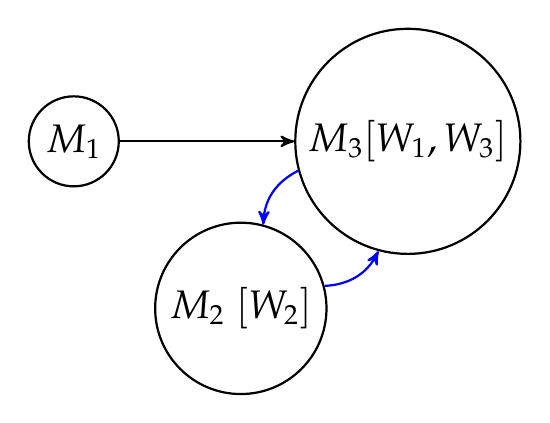
\begin{tikzpicture}[->,>=stealth',auto,node distance=3cm,
  thick,main node/.style={circle,draw,font=\sffamily\Large\bfseries}]

  \node[main node] (1) {$M_1$};
  \node[main node] (2) [below right of=1] {$M_2$ $[W_2]$};
  \node[main node] (3) [above right of=2] {$M_3[W_1, W_3]$};
  
 %\node[main node] (4) [right of=3] {d};

% [->,>=stealth',auto,node distance=1mm,
%   thick,main node/.style={[],draw,font=\sffamily\small}]

%   \node[main node] (4) [below of=2] {$W_2$};

  \path[every node/.style={font=\sffamily\small}]
    (1) edge node [ right] {} (3)
    (2) edge[blue, bend right]  node [right] {} (3)
    (3) edge[blue, bend right] node [right] {} (2);
%    (3) edge node [right] {} (4)
 %   (4) edge[bend right] node [left] {} (1);
% \node [below=1.5cm] at (2)
 %       {\textbf{Step 1} };
\end{tikzpicture}
\end{center}
A cycle exists between $M_2$ and $M_3$, therefore exchange of endowments occur, $M_2$ and $M_3$ are matched with $W_3$ and $W_2$ respectively.\\
Having no other choice, $M_1$ gets matched with $W_1$.

$\therefore$ The final matchings are {$M_1:W_1, M_2:W_3, M_3:W_2$}.

We notice that even though the matching is \textit{unstable}, it is still Pareto optimal from the men's side.

\subsection{Serial Dictatorship (SD)}

 The \textbf{Serial Dictatorship (SD)} mechanism is a method for allocating individuals or agents to each other based on their preferences in a one-by-one sequential manner. It involves a sequence of "dictators" who have the authority to make decisions and determine the pairings or matchings. The serial dictatorship with a fixed priority is strategy-proof and efficient.

\textbf{Example :} Consider the preference profile at \ref{preference}, applying SD with priority sequence as $M_1 \rightarrow M_2 \rightarrow M_3$.\\
\begin{center}
    \textbf{Step 1 :} $M_1$ gets matched to $W_3$.\\
    \textbf{Step 2 :} $M_2$ gets matched to $W_2$.\\
    \textbf{Step 3 :} $M_3$ gets matched to $W_1$.\\
\end{center}

Serial Dictatorship is \textit{strategy proof} from men's side but may produce \textit{unstable} matching.

\section{R code for the three algorithms}
 \begin{center}
        \textbf{Deferred Acceptance}
    \lstinputlisting[language=R]{Deffered_Acceptance.R}

    \textbf{Top Trading Cycle}
    \lstinputlisting[language=R]{TTC.R}
    \textbf{Serial Dictatorship}
    \lstinputlisting[language=R]{Serial_Dictatorship.R}
\end{center}

\section{Our Contribution}

In this work, we intend to compare the three algorithms based on some criteria that, in some sense, take into account the utilities the agents (men and women) get from the algorithm across profiles. One such natural measure is expected rank utility. Although this notion is less explored in the literature, it is intuitive and simple to understand and interpret. Below we discuss it in detail with the help of a few definitions.

For a matching $\mu$ at a preference profile $(\succ,\rva)$, the rank utility of a person (a man or a woman) is $n+1$ minus the rank of their partner in the matching. Mathematically, for a man $M$, the rank utility is $n+1-r(\mu(M),\succ_M)$ and for a woman $W$, it is   $n+1-r(\mu^{-1}(W),\rva_W)$. Note that the rank utility of a person is proportional to the rank of their partner, the higher ranked partner someone gets, the more utility they get. The total rank utility at a preference profile is the sum of the rank utilities of all men and women, i.e., $\sum_{M\in \pmb{M}}[n+1-r(\mu(M),\succ_M)]+\sum_{W\in \pmb{W}}[n+1-r(\mu^{-1}(W),\rva_W)]$. Finally, for a matching function, to combine the utilities across different profiles, we assume a probability distribution over the preference profiles and compute the expectation of the rank utility under this probability distribution. Let $p:\mathbb{L}(\pmb{M})^n \cup \mathbb{L}(\pmb{W})^n\to [0,1]$ be a pmf on the set of preference profiles, then for a matching function $f$, the expected rank utility w.r.t. $p$ is given by
$$\sum_{[(\succ,\rva)\in \mathbb{L}(\pmb{M})^n \cup \mathbb{L}(\pmb{W})^n]} \left[\sum_{M\in \pmb{M}}[n+1-r(\mu(M),\succ_M)]+\sum_{W\in \pmb{W}}[n+1-r(\mu^{-1}(W),\rva_W)]\right]p((\succ,\rva)).$$

\subsection{A particular case when $n=3$ and $p$ is uniform}
To start with, we assume $n=3$ and $p$ is uniform and compare the three algorithms in terms of their expected rank utilities. Note that under the uniform distribution, it's equivalent to taking the sum of the rank utilities across different profiles. To get some idea about the comparison, We first compute the total rank utilities of three algorithms using R. You may find the code below. 

\subsubsection{Findings using R code}

    The below function was used to calculate the score of men and women given their preferences and current match as input.
    \lstinputlisting[language=R]{Score_Function.R}

    \begin{center}
        Main Function
    \end{center}
    The below code was used to call and run all the functions(DA, TTC and SD) and calculate and store their score using the \textit{Score Function}.\\
    Here, we see that the total possible preferences in the case of 4 men and women case will be ${4!}^8$, which is approximately equal to $10^{11}$, and as we increase the number of men and women, total cases will increase drastically, making it computationally inefficient to consider each case.\\
    $\therefore$ For $n \geq 4$, we did random sampling to get preference profiles of men and women and ran the loop for $10^6$ times and took average of it to get the mean score.
    \lstinputlisting[language=R, firstline=3, lastline=58]{Game_Theory.R}

    After running simulations and observing them we hypothesized the following statements:
    \begin{enumerate}
        \item According to total rank-utility, Deferred Acceptance is the best algorithm among Deferred acceptance, TTC, and serial dictatorship.
        \item If we only consider the Men’s Side while calculating rank-utility, TTC with women as objects is the best algorithm.
    \end{enumerate}

    
\subsubsection{Results}

In this section, we mathematically prove the findings, we get using R code in the previous section. We start with a Lemma that states an interesting fact about TTC and DA. At any profile, if a man is matched to his  last-ranked women in DA, he will be matched with the same woman in TTC as well.  

\begin{lemma}\label{lem_1}
 If a man is assigned to his last-ranked
 women in DA, then he will have the same assignment in TTC.
 \end{lemma}
    
% \documentclass{article}
% \usepackage[english]{babel}
% \usepackage[a4paper,margin=1in,footskip=0.25in]{geometry}
% \usepackage{amssymb,amsmath,latexsym,color,amsthm,authblk,mathpazo,palatino,bbding,setspace,datetime,breakcites,hyphenat,microtype,diagbox,tikz,xcolor,tkz-graph,subcaption,graphicx,titlesec,amsbsy, listings}
% \usepackage{titlesec}
% \usepackage{mathptmx}
% %\usepackage{times}
% %\usepackage{cite}
% \usepackage[round,authoryear]{natbib}
% \citestyle{authordate}
% \usepackage{hyperref,theoremref}
% \usepackage[titletoc,title]{appendix}
% %\usepackage[author={Souvik Roy}]{pdfcomment}
% %\usepackage{parskip}
% \usepackage[shortlabels]{enumitem}
% \usepackage{float}
% \usepackage{amssymb}
% \restylefloat{table}
% \everymath{\displaystyle}
% \usepackage{pstricks}

% \usepackage{tikz}
% \usetikzlibrary{arrows}


% %\usepackage{accents}
% %\setlength{\parindent}{15pt}
% \usepackage{accents}

% \newcommand{\ut}[1]{\underaccent{\tilde}{#1}}
% \renewcommand{\vec}[1]{\ut{#1}}

% \definecolor{armygreen}{rgb}{0.29, 0.8, 0.13}
% \definecolor{auburn}{rgb}{0.43, 0.21, 0.1}
% \definecolor{burgundy}{rgb}{0.5, 0.0, 0.13}
% \definecolor{medium red}{rgb}{.490,.298,.337}
% \definecolor{dark red}{rgb}{.235,.141,.161}

% \hypersetup{
% 	colorlinks = true,
% 	linkcolor = {burgundy},
% 	citecolor = {burgundy}, 		
% 	linkbordercolor = {white},
% }

% \captionsetup[sub]{font=scriptsize}

% % Page length commands go here in the preamble
% %\setlength{\oddsidemargin}{-0.25in} % Left margin of 1 in + 0 in = 1 in
% %\setlength{\textwidth}{7in}   % Right margin of 8.5 in - 1 in - 6.5 in = 1 in
% %\setlength{\topmargin}{-.75in}  % Top margin of 2 in -0.75 in = 1 in
% %\setlength{\textheight}{9.5in}  % Lower margin of 11 in - 9 in - 1 in = 1 in

% \interfootnotelinepenalty=10000
% \raggedbottom

% \let\OLDthebibliography\thebibliography
% \renewcommand\thebibliography[1]{
% 	\OLDthebibliography{#1}
% 	\setlength{\parskip}{0pt}
% 	\setlength{\itemsep}{0pt plus 0.1ex}
% }

% \newcommand{\va}{\vartriangleleft}
% \newcommand{\vaq}{\trianglelefteq}
% \newcommand{\rva}{\vartriangleright}
% \newcommand{\rvaq}{\trianglerighteq}


% \DeclareFontFamily{U}{mathx}{\hyphenchar\font45}
% \DeclareFontShape{U}{mathx}{m}{n}{<-> mathx10}{}
% \DeclareSymbolFont{mathx}{U}{mathx}{m}{n}
% \DeclareMathAccent{\widebar}{0}{mathx}{"73}

% \titleformat{\section}[block]{\normalfont\scshape\large\filcenter}{\thesection .}{1em}{}
% \titleformat{\subsection}{\normalfont\scshape\large}{\thesubsection}{1em}{}
% \titleformat{\subsubsection}{\normalfont\scshape\large}{\thesubsubsection}{1em}{}
% \titleformat{\paragraph}
% {\normalfont\scshape\large}{\theparagraph}{1em}{}
% \titlespacing*{\paragraph}
% {0pt}{3.25ex plus 1ex minus .2ex}{1.5ex plus .2ex}

% % Theorem Styles
% \newtheorem{theorem}{Theorem}
% \newtheorem{proposition}{Proposition}
% \newtheorem{claim}{Claim}
% \newtheorem{lemma}{Lemma}
% \newtheorem{corollary}{Corollary}
% \newtheorem{observation}{Observation}[section]
% % Definition Styles
% \theoremstyle{definition}
% \newtheorem{definition}{Definition}[section]
% \newtheorem{example}{Example}[section]
% \theoremstyle{remark}
% \newtheorem{remark}{\textsc{Remark}}[section]

% \renewenvironment{proof}[1][\proofname]{{\bfseries #1: }}{\qed}
% \newcommand{\tbf}{\textbf}
% \newcommand{\sr}{\textcolor{red}}
% \newcommand{\srs}{\textcolor{blue}}
% \newcommand{\srsk}{\textcolor{armygreen}}
% \newdateformat{monthyeardate}{\monthname[\THEMONTH], \THEYEAR}
%\begin{document}

\begin{proof}
Let $(\succ,\rva)$ be a preference profile where for all $i\in \{1,2,3\}$, $M_i$ has preference $\succ_i$ and $W_i$ has preference $\rva_i$, and $M_1$ is matched to her third preferred women in DA. Without loss of generality, let's assume $W_1 \succ_1 W_2 \succ_1 W_3$, and $M_2$ and $M_3$ are matched with $W_1$ and $W_2$, respectively in DA. Since the outcome of DA is stable, $W_1$ must prefer $M_2$ over $M_1$ and $W_2$ must prefer $M_3$ over $M_1$. Therefore, we have \[  \begin{array}{c}
	   \rva_1 \\
	\hline
	\vdots \\
	M_2\\
        \vdots\\
        M_1\\
        \vdots
\end{array} 
\hspace{10mm}
%
\begin{array}{c}
	\rva_2 \\
	\hline
	\vdots \\
	M_3\\
        \vdots\\
        M_1\\
        \vdots
\end{array} 
\]
Further, $M_2$ will prefer $W_1$ over $W_3$ and $M_3$ will prefer $W_2$ over $W_3$. To see this, assume for contradiction  $M_2$ prefers $W_3$ over $W_1$. Since finally $M_2$ is matched with $W_1$, it means at some stage of the algorithm (say $t^{th}$ stage), $M_2$'s proposal to $W_3$ got rejected. Suppose $M_1$'s proposal to $W_3$ caused this rejection. Since $W_3$ is $M_1$'s least preferred woman, it must be that he had already proposed to $W_1$ and $W_2$. Therefore, by DA algorithm, $W_1$ and $W_2$ had at least one proposal at $t^{th}$ stage. But this is a contradiction as $W_3$ had two proposals at $t^{th}$ stage. Now assume $M_3$'s proposal to $W_3$ caused the rejection of $M_2$'s proposal to $W_3$ at the $t^{th}$ stage. Since finally $M_3$ is matched with $W_2$, it means, at some later stage, his proposal to $W_3$ also got rejected. But this rejection can only cause due to $M_1$'s proposal to $W_3$, which again means, at that stage, $W_3$ had two proposals, a contradiction. Thus, we have

% Consider the following matching, $M_1$ is matched with $W_1$, $M_2$ is matched with $W_3$, and $M_3$ is matched with $W_2$. We claim that this matching is stable. As $M_1$ is getting his top-women, he will not be in a blocking pair. Suppose $M_2$ blocks with $W_2$. This means $M_2$ prefers $W_2$ over $W_3$, hence the most, and $W_2$ prefers $M_2$ over $M_3$, hence, the most. But this contradicts as they are not matched in DA. Finally, suppose $M_3$ blocks with either $W_1$ or $W_3$. 


\[  \begin{array}{c}
	\succ_2 \\
	\hline
	\vdots \\
	W_1\\
        \vdots\\
        W_3\\
        \vdots
\end{array} 
\hspace{10mm}
%
\begin{array}{c}
	\succ_3 \\
	\hline
	\vdots \\
	W_2\\
        \vdots\\
        W_3\\
        \vdots
\end{array} 
\]
We claim that, in TTC, $M_1$ will be matched with $W_3$. Note that $M_2$ and $M_3$ have either $W_1$ or $W_2$ as their top preferred women. Moreover, $W_1$ and $W_2$ have either $M_2$ or $M_3$ as their top-preferred men. Therefore, in the first step of TTC, either they will point towards each other, or they will point towards themselves, or they both will point to either $M_2$ or $M_3$. 
If they both point to each other or themselves, they will get matched to $W_1$ and $W_2$, and as a result, $M_1$ will go with $W_3$. So, assume they both point to one of them. Since, in DA, $M_2$ got matched with $W_1$ and $M_3$ is matched with $W_2$, this means either both point to $M_2$ and $W_1$ is with $M_2$ initially, or both point to $M_3$ and $W_2$ is with $M_3$ initially. Suppose both point to $M_2$ and $W_1$ is with $M_2$ initially. Hence, $M_2$ will be matched with $W_1$. Further, as $M_3$ prefers $W_2$ over $W_3$ and $W_2$ prefers $M_3$ over $M_1$, $M_3$ will be matched to $W_2$ in the second round implying $M_1$ will be matched with $W_3$. The argument is similar when both point to $M_3$ and $W_2$ is with $M_3$ initially. This completes the proof of the lemma.
\end{proof}

% Suppose not, and first assume that $M_1$ is matched with $W_1$. Since $W_1$ prefers $M_2$ over $M_1$, by the TTC algorithm,  it necessarily means $M_2$ is matched with someone whom he prefers over $W_1$. Thus, $M_2$ is matched with $W_2$ in TTC, and hence, $M_3$ is matched with $W_3$. Also, as $M_3$ prefers $W_2$ over $W_3$, his match in the algorithm, it must be that $W_2$ prefers her match over $M_3$. This means $M_2\rva_2 M_3$. Combining all these observations, we have

% \[  \begin{array}{c}
% 	   \rva_2 \\
% 	\hline
% 	M_2\\
%         M_3\\
%         M_1\\
% \end{array} 
% \hspace{10mm}
% %
% \begin{array}{c}
% 	\succ_2 \\
% 	\hline
% 	W_2 \\
% 	W_1\\
%         W_3\\
% \end{array} 
% \]

% % and \[  \begin{array}{c}
% % 	\succ_2 \\
% % 	\hline
% % 	\vdots \\
% % 	W_1\\
% %         \vdots\\
% %         W_3\\
% %         \vdots
% % \end{array} 
% % \hspace{10mm}
% % %
% % \begin{array}{c}
% % 	\succ_3 \\
% % 	\hline
% % 	\vdots \\
% % 	W_2\\
% %         \vdots\\
% %         W_3\\
% %         \vdots
% % \end{array} 
% % \]


% % $M_1$, $M_2$, and $M_3$ have preferences $\succ_1$, $\succ_2$, and $\succ_3$, respectively, and $W_1$, $W_2$, and $W_3$ have preferences $\rva_1$, $\rva_2$, and $\rva_3$, respectively. Without loss of generality $W_1 \succ_1 W_2 \succ_1 W_3$.


% Without loss of generality assume that $M_1$ has the preference $\succ_1$ where  $W_1 \succ_1 W_2 \succ_1 W_3$. If $M_1$ is getting his third preferred woman ($W_3$) in DA, it means he got rejected by the top two women in his preference in the algorithm. Therefore, three cases are possible. We consider them separately below.

% \noindent\textbf{Case I :-} All men have  $W_1$ as their first preferred women.

% Now applying DA;
% $$\textbf{Step 1}: M_1, M_2, M_3 \text{ proposes } W_1$$
% For $W_1$ to reject $M_1$, one of ${M_2, M_3}$ must be above $M_1$ in her preference profile.  Without loss of generality, assume $M_2$ to be  the first preference of  $W_1$.  Therefore preference profile of 
% \begin{equation}
% W_1 = (M_2 \succ ... ) \label{eq1}
% \end{equation}

% \begin{center}$\therefore$ $W_1$ reject both $M_1$ and $M_3$.\end{center}

% Now, for $M_1$ to get rejected by his $2^{nd}$ preferred women $M_3$ must also propose $W_2$ and get accepted by her. Therefore, preference profile of  \begin{equation}W_2 = (... M_3 \succ ... M_1 \succ...)\label{eq2}\end{equation}

% \begin{center}\textbf{Step 2 :}$W_2$ accepts $M_3$ and rejects $M_1$\end{center}
% $$\textbf{Step 3 :} M_1 \text{ proposes } W_3$$

% Not getting any other proposals, she accepts $M_1$, and $M_1$ gets paired with his third preferred woman.

% By using \eqref{eq1} and \eqref{eq2}, we can make a preference profile table of all men and women; 
% \begin{center}
% \begin{tabular}{ c|c|c } 
 
%  $M_1$ & $M_2$ & $M_3$  \\ 
% \hline
%  $W_1$ & $W_1$ & $W_1$ \\ 
%  $W_2$ & : & $W_2$ \\ 
%  $W_3$ & : & :\\

% \end{tabular}
% \begin{tabular}{ c|c|c } 
 
%  $W_1$ & $W_2$ & $W_3$  \\ 
% \hline
%  $M_2$ & : & :\\ 
%  : & $M_3$ & :\\ 
%  : & : & :\\
%   & $M_1$ & \\
%   & : & \\

% \end{tabular}
% \end{center}
% Now, we apply TTC by constructing a directed graph with 3 vertices, one for each man and putting a directed edge from vertex of men i to vertex of men j if the top-ranked object of men i is endowed with
% men j.\\
% In each graph, men who are part of the \textit{cycle with blue edges} can trade their endowments.
% \\
% \begin{center}
% \begin{tikzpicture}[->,>=stealth',auto,node distance=3cm,
%   thick,main node/.style={circle,draw,font=\sffamily\Large\bfseries}]

%   \node[main node] (1) {$M_1$};
%   \node[main node] (2) [below right of=1] {$M_2$ $[W_1]$};
%   \node[main node] (3) [above right of=2] {$M_3$};
  
%  %\node[main node] (4) [right of=3] {d};

% % [->,>=stealth',auto,node distance=1mm,
% %   thick,main node/.style={[],draw,font=\sffamily\small}]

% %   \node[main node] (4) [below of=2] {$W_2$};

%   \path[every node/.style={font=\sffamily\small}]
%     (1) edge node [right] {} (2)
%     (2) edge[blue] [loop right] node [right] {} (2)
%     (3) edge node [left] {} (2);
% %    (3) edge node [right] {} (4)
%  %   (4) edge[bend right] node [left] {} (1);
% % \node [below=1.5cm] at (2)
%  %       {\textbf{Step 1} };
% \end{tikzpicture}
% \end{center}
% Here, we see that there is only one cycle involving
% $M_2$. Therefore, $M_2$ gets paired with $W_1$.
% \\

% \begin{center}
% \begin{tikzpicture}[->,>=stealth',auto,node distance=3cm,
%   thick,main node/.style={circle,draw,font=\sffamily\Large\bfseries}]

%   \node[main node] (1) {$M_1$};
%   \node[main node] (3) [right of=1] {$M_3[W_2]$};
  
%  %\node[main node] (4) [right of=3] {d};

% % [->,>=stealth',auto,node distance=1mm,
% %   thick,main node/.style={[],draw,font=\sffamily\small}]

% %   \node[main node] (4) [below of=2] {$W_2$};

%   \path[every node/.style={font=\sffamily\small}]
%     (1) edge node [right] {} (3)
%     (3) edge[blue, loop right] node [right ] {} (3);
% %    (3) edge node [right] {} (4)
%  %   (4) edge[bend right] node [left] {} (1);
% % \node [below=1.5cm] at (2)
%  %       {\textbf{Step 1} };
% \end{tikzpicture}
% \end{center}
% Here also, we see that there is only one cycle involving
% $M_3$. Therefore, $M_3$ gets paired with $W_2$.
% \\
% $\therefore$ With no other choice left \textbf{$M_1$ gets paired to $W_3$} (\textit{his third preference}).
% \\ \\


% \textbf{Case II :-} $M_2$ and $M_3$ have $M_1$'s second preffered woman( i.e. $W_2$) as their first preference.

% Now, applying DA;
% $$
% \textbf{Step 1}
% \begin{cases}
% {M_1} \text{ proposes} W_1 \\
% {M_2, M_3} \text{ proposes} W_2
% \end{cases}
% $$
% Without loss of generality, let us assume that $M_3$ gets rejected by $W_2$, which means $M_3$ is somewhere below $M_2$ in $W_2$ preference. i.e.  \begin{equation}W_2 = (M_2 \succ ...)\label{eq3}\end{equation}

% Now if $M_3$ were to propose $W_2$, $M_1$ will be paired with $W_1$, which is not something we want, so in order for $M_1$ to form pair with $W_3$, $M_3$ must propose $W_1$ ans she must accept his proposal. 

% Therefore, preference profile of \begin{equation}W_1 = (... M_3 \succ ... M_1 \succ...)\label{eq4}\end{equation}

% $$\textbf{Step 2 :} M_3 \text{ proposes }W_1$$
% $\therefore$$W_1$ accepts $M_3$ and rejects $M_1$

% $$\textbf{Step 3 :}M_1 \text{ proposes }W_2$$
% As $W_2$ already got a proposal from her top pref $M_2$, therefore she'll reject $M_1$.
% $$\textbf{Step 4 :} M_1 \text{ proposes } W_3$$
% With no other proposals, she'll accept $M_1$. With this, $M_1$ is finally paired with his third preference, $W_3$.

% By using \eqref{eq3} and \eqref{eq4}, we can make a preference profile table of all men and women; 
% \begin{center}
% \begin{tabular}{ c|c|c } 
 
%  $M_1$ & $M_2$ & $M_3$  \\ 
% \hline
%  $W_1$ & $W_2$ & $W_2$ \\ 
%  $W_2$ & : & $W_1$ \\ 
%  $W_3$ & : & :\\

% \end{tabular}
% \begin{tabular}{ c|c|c } 
 
%  $W_1$ & $W_2$ & $W_3$  \\ 
% \hline
%  : &  & \\ 
%  $M_3$ & $M_2$ & :\\ 
%  : & : & :\\
%   $M_1$& : & :\\
%  : &  & \\

% \end{tabular}
% \end{center}
% \\
% Now, we apply TTC by constructing a directed graph with 3 vertices, one for each man and putting a directed edge from vertex of men i to vertex of men j if the top-ranked object of men $i$ is endowed with
% men $j$.

% In each graph, men who are part of the \textit{cycle with blue edges} can trade their endowments.
% \\


% \begin{center}
% \begin{tikzpicture}[->,>=stealth',auto,node distance=3cm,
%   thick,main node/.style={circle,draw,font=\sffamily\Large\bfseries}]

%   \node[main node] (1) {$M_1$};
%   \node[main node] (2) [below right of=1] {$M_2$ $[W_2]$};
%   \node[main node] (3) [above right of=2] {$M_3[W_1]$};
  
%  %\node[main node] (4) [right of=3] {d};

% % [->,>=stealth',auto,node distance=1mm,
% %   thick,main node/.style={[],draw,font=\sffamily\small}]

% %   \node[main node] (4) [below of=2] {$W_2$};

%   \path[every node/.style={font=\sffamily\small}]
%     (1) edge[bend left] node [ right] {} (3)
%     (2) edge[blue] [loop left] node [left] {} (2)
%     (3) edge node [left] {} (2);
% %    (3) edge node [right] {} (4)
%  %   (4) edge[bend right] node [left] {} (1);
% % \node [below=1.5cm] at (2)
%  %       {\textbf{Step 1} };
% \end{tikzpicture}
% \end{center}
% It doesn't matter among $M_3, M_2$ who is at top preference of $W_1$ as we see that there is only one cycle involving $M_2$. Therefore, $M_2$ gets paired with $W_1$.

% \begin{center}
% \begin{tikzpicture}[->,>=stealth',auto,node distance=3cm,
%   thick,main node/.style={circle,draw,font=\sffamily\Large\bfseries}]

%   \node[main node] (1) {$M_1$};
%   \node[main node] (3) [right of=1] {$M_3[W_1]$};
  
%  %\node[main node] (4) [right of=3] {d};

% % [->,>=stealth',auto,node distance=1mm,
% %   thick,main node/.style={[],draw,font=\sffamily\small}]

% %   \node[main node] (4) [below of=2] {$W_2$};

%   \path[every node/.style={font=\sffamily\small}]
%     (1) edge node [right] {} (3)
%     (3) edge[blue, loop right] node [right] {} (3);
% %    (3) edge node [right] {} (4)
%  %   (4) edge[bend right] node [left] {} (1);
% % \node [below=1.5cm] at (2)
%  %       {\textbf{Step 1} };
% \end{tikzpicture}
% \end{center}
% Here also, we see that there is only one cycle involving $M_3$. Therefore, $M_3$ gets paired with $W_1$.\\
% $\therefore$ With no other choice left \textbf{$M_1$ gets paired to $W_3$}(\textit{his third preference}).
% \\
% \\
% \textbf{Case III :- } One of the men has $W_1$ as his first preference and other has $W_2$ as his first preference.

% Without loss of generality, assuming the preferences of all men be:

% \begin{center}
%     \begin{tabular}{c|c|c}
%         $M_1$ & $M_2$ & $M_3$ \\
%         \hline
%         $W_1$ & $W_1$ & $W_2$ \\
%         $W_2$ & :   &   : \\
%         $W_3$ & :   &   :
%     \end{tabular}
% \end{center}

% A few things required to have $M_1$ get paired with his third preference are:
% \begin{itemize}
%     \item $W_2$ must prefer $M_3$ over $M_1$ as to reject $M_1$ later.
%     \item $W_1$ must prefer $M_2$ over $M_1$ as to reject $M_1$ at forst step of DA.
% \end{itemize}
% Keeping above things in mind preferences of women will look like:

% \begin{center}
%     \begin{tabular}{c|c|c}
%         $W_1$ & $W_2$ & $W_3$ \\
%         \hline
%           :   &   :   &   \\
%         $M_2$ & $M_3$ & : \\
%           :   &   :   & : \\
%         $M_1$ & $M_1$ & : \\
%           :   &   :   &   
%     \end{tabular}
% \end{center}

% On the basis of preferences of $W_1$ and $W_2$, assignment through TTC will progress differently, so we will make cases and see the result of TTC over different preferences of $W_1$ and $W_2$  :

% \textbf{a)}
% \begin{center}
%     \begin{tabular}{c|c|c}
%         $W_1$ & $W_2$ & $W_3$ \\
%         \hline
%           $M_3$   &  $M_2$   & :  \\
%         $M_2$ & $M_3$ & : \\
%         $M_1$ & $M_1$ & : \\
%     \end{tabular}
% \end{center}

% Applying TTC;

% \begin{center}
% \begin{tikzpicture}[->,>=stealth',auto,node distance=3cm,
%   thick,main node/.style={circle,draw,font=\sffamily\Large\bfseries}]

%   \node[main node] (1) {$M_1$};
%   \node[main node] (2) [below right of=1] {$M_2[W_2]$};
%   \node[main node] (3) [above right of=2] {$M_3[W_1]$};
  
%  %\node[main node] (4) [right of=3] {d};

% % [->,>=stealth',auto,node distance=1mm,
% %   thick,main node/.style={[],draw,font=\sffamily\small}]

% %   \node[main node] (4) [below of=2] {$W_2$};

%   \path[every node/.style={font=\sffamily\small}]
%     (1) edge[bend left] node [ right] {} (3)
%     (2) edge[blue] [bend left] node [right] {} (3)
%     (3) edge[blue, bend left] node [right] {} (2);
% %    (3) edge node [right] {} (4)
%  %   (4) edge[bend right] node [left] {} (1);
% % \node [below=1.5cm] at (2)
%  %       {\textbf{Step 1} };
% \end{tikzpicture}
% \end{center}
% A cycle exists between $M_2 \& M_3$. Therefore, $M_2$ gets paired to $W_1$, while  $M_3$ gets paired to $W_2$.
% \\ \\
% The only women left unmatched is $W_3$, so \textbf{$M_1$ gets paired with $W_3$}.\\

% \textbf{b)}
% \begin{center}
%     \begin{tabular}{c|c|c}
%         $W_1$ & $W_2$ & $W_3$ \\
%         \hline
%         $M_3$ & $M_3$   & :  \\
%         $M_2$ & : & : \\
%         $M_1$ & : & : \\
%     \end{tabular}
% \end{center}

% Applying TTC;
% \begin{center}
% \begin{tikzpicture}[->,>=stealth',auto,node distance=3cm,
%   thick,main node/.style={circle,draw,font=\sffamily\Large\bfseries}]

%   \node[main node] (1) {$M_1$};
%   \node[main node] (2) [below right of=1] {$M_2$};
%   \node[main node] (3) [above right of=2] {$M_3[W_1, W_2]$};
  
%  %\node[main node] (4) [right of=3] {d};

% % [->,>=stealth',auto,node distance=1mm,
% %   thick,main node/.style={[],draw,font=\sffamily\small}]

% %   \node[main node] (4) [below of=2] {$W_2$};

%   \path[every node/.style={font=\sffamily\small}]
%     (1) edge node [ right] {} (3)
%     (2) edge node [right] {} (3)
%     (3) edge[blue, loop right] node [right] {} (2);
% %    (3) edge node [right] {} (4)
%  %   (4) edge[bend right] node [left] {} (1);
% % \node [below=1.5cm] at (2)
%  %       {\textbf{Step 1} };
% \end{tikzpicture}
% \end{center}
% Here, we see there is only one cycle involving $M_3$. Therefore, $M_3$ gets paired with $W_2$.

% \begin{center}
% \begin{tikzpicture}[->,>=stealth',auto,node distance=3cm,
%   thick,main node/.style={circle,draw,font=\sffamily\Large\bfseries}]

%   \node[main node] (1) {$M_1$};
%   \node[main node] (2) [right of=1] {$M_2[W_1]$};
  
%  %\node[main node] (4) [right of=3] {d};

% % [->,>=stealth',auto,node distance=1mm,
% %   thick,main node/.style={[],draw,font=\sffamily\small}]

% %   \node[main node] (4) [below of=2] {$W_2$};

%   \path[every node/.style={font=\sffamily\small}]
%     (1) edge node [ right] {} (2)
%     (2) edge[blue, loop right] node [right] {} (2);
% %    (3) edge node [right] {} (4)
%  %   (4) edge[bend right] node [left] {} (1);
% % \node [below=1.5cm] at (2)
%  %       {\textbf{Step 1} };
% \end{tikzpicture}
% \end{center}
% Here, a cycle involving $M_2$ exists. Therefore, $M_2$ gets paired with $W_1$.
% \\ \\
% The only women left unmatched is $W_3$, so \textbf{$M_1$ gets paired with $W_3$}.\\

% \textbf{c)}
% \begin{center}
%     \begin{tabular}{c|c|c}
%         $W_1$ & $W_2$ & $W_3$ \\
%         \hline
%           $M_2$   & $M_2$   & :  \\
%                 : & $M_3$ & : \\
%                 : & $M_1$ & : \\
%     \end{tabular}
% \end{center}


% Applying TTC;
% \begin{center}
% \begin{tikzpicture}[->,>=stealth',auto,node distance=3cm,
%   thick,main node/.style={circle,draw,font=\sffamily\Large\bfseries}]

%   \node[main node] (1) {$M_1$};
%   \node[main node] (2) [below right of=1] {$M_2[W_1, W_2]$};
%   \node[main node] (3) [above right of=2] {$M_3$};
  
%  %\node[main node] (4) [right of=3] {d};

% % [->,>=stealth',auto,node distance=1mm,
% %   thick,main node/.style={[],draw,font=\sffamily\small}]

% %   \node[main node] (4) [below of=2] {$W_2$};

%   \path[every node/.style={font=\sffamily\small}]
%     (1) edge node [ right] {} (2)
%     (2) edge[blue, loop right] node [right] {} (2)
%     (3) edge node [right] {} (2);
% %    (3) edge node [right] {} (4)
%  %   (4) edge[bend right] node [left] {} (1);
% % \node [below=1.5cm] at (2)
%  %       {\textbf{Step 1} };
% \end{tikzpicture}
% \end{center}
% Here, we see there is only one cycle involving $M_2$. Therefore, $M_2$ gets paired with $W_1$.

% \begin{center}
% \begin{tikzpicture}[->,>=stealth',auto,node distance=3cm,
%   thick,main node/.style={circle,draw,font=\sffamily\Large\bfseries}]

%   \node[main node] (1) {$M_1$};
%   \node[main node] (3) [right of=1] {$M_3[W_2]$};
  
%  %\node[main node] (4) [right of=3] {d};

% % [->,>=stealth',auto,node distance=1mm,
% %   thick,main node/.style={[],draw,font=\sffamily\small}]

% %   \node[main node] (4) [below of=2] {$W_2$};

%   \path[every node/.style={font=\sffamily\small}]
%     (1) edge node [ right] {} (3)
%     (3) edge[blue, loop right] node [right] {} (3);
% %    (3) edge node [right] {} (4)
%  %   (4) edge[bend right] node [left] {} (1);
% % \node [below=1.5cm] at (2)
%  %       {\textbf{Step 1} };
% \end{tikzpicture}
% \end{center}
% Here, a cycle involving $M_3$ exists. Therefore, $M_3$ gets paired with $W_2$.
% \\ \\
% The only women left unmatched is $W_3$, so \textbf{$M_1$ gets paired with $W_3$}.\\

% \textbf{d)}
% \begin{center}
%     \begin{tabular}{c|c|c}
%         $W_1$ & $W_2$ & $W_3$ \\
%         \hline
%           $M_2$   & $M_3$   & :  \\
%                 : & : & : \\
%                 : & : & : \\
%     \end{tabular}
% \end{center}

% Applying TTC;
% \begin{center}
% \begin{tikzpicture}[->,>=stealth',auto,node distance=3cm,
%   thick,main node/.style={circle,draw,font=\sffamily\Large\bfseries}]

%   \node[main node] (1) {$M_1$};
%   \node[main node] (2) [below right of=1] {$M_2[W_1]$};
%   \node[main node] (3) [above right of=2] {$M_3[W_2]$};
  
%  %\node[main node] (4) [right of=3] {d};

% % [->,>=stealth',auto,node distance=1mm,
% %   thick,main node/.style={[],draw,font=\sffamily\small}]

% %   \node[main node] (4) [below of=2] {$W_2$};

%   \path[every node/.style={font=\sffamily\small}]
%     (1) edge node [ right] {} (2)
%     (2) edge[blue, loop right] node [right] {} (2)
%     (3) edge[blue, loop right] node [right] {} (3);
% %    (3) edge node [right] {} (4)
%  %   (4) edge[bend right] node [left] {} (1);
% % \node [below=1.5cm] at (2)
%  %       {\textbf{Step 1} };
% \end{tikzpicture}
% \end{center}
% Here, we see there exist 2 different cycles involving $M_2 \& M_3$ separately. Therefore, $M_2:W_1$, and $M_3:W_2$ gets paired.
% \\  \\
% The only women left unmatched is $W_3$, so \textbf{$M_1$ gets paired with $W_3$}.\\ \\
% \\
% $\therefore$ In all three cases, we see that if $M_1$ gets his third preference in DA, then \textbf{$M_1$ will always get the third preference using TTC}.

%\end{proof}
%\end{document}

We have not been able to prove completely the findings mentioned in the previous section. In the following, we briefly describe our work plan for the future. Note that Lemma \ref{lem_1} immediately implies that if, at a preference profile, a man has more rank utility in TTC than in DA, it must be that he is getting his top-preferred woman in TTC and his second preferred woman in DA. We will use this fact to characterize the profiles where the total rank-utility of the men is strictly more in TTC than DA. Further, we will show that if, at a profile, TTC dominates DA with respect to the total rank-utility, it must be the case that the total rank-utility of the men is strictly more in TTC than DA. Thus, it's enough to characterize the profiles where TTC dominates DA in terms of their total rank-utility for the men. 
 



% \begin{itemize}
    
%     \item \textbf{Mechanism Design:} A planner needs to design a mechanism where strategic agents can interact. The interactions of agents result in some outcomes. While there are several possible ways to design the rules of the mechanism, the planner has a particular objective in mind. For example, the objective can be \textit{utilitarian}(maximization of the total utility of agents) or \textit{maximization of his own utility} or some fairness objective. Depending on the objective, the mechanism needs to be designed in a manner such that when strategic agents interact, the resulting outcome gives the desired objective. One can think of mechanism design as the reverse engineering of game theory.
    
%     \item \textbf{Matching theory} refers to theory of a rich class of models where there are two “sides” and one side is matched to the other.

%      \item \textbf{Matching} is the process of pairing or connecting items or entities from two or more sets based on predetermined criteria or preferences. It entails establishing relationships or associations between elements so as to optimize certain objectives or satisfy desired conditions.

%      \item A \textbf{social choice function} $f$ is a mapping $f : \mathbb{W}^n$ $\rightarrow$  $A$, where $\mathbb{W}^n$ represents the set of all preference ordering over $W$(set of all women), and $A$ represents set of alternatives { \textit{feasible matching}, i.e., an injective mapping from $M$(set of all men) to $W$}. We denote by $f(\succ)$ the matching produced at a preference profile $\succ$. We denote by $f_i(\succ)$ the assignment of agent i at a preference profile $\succ$. 

%      \item A social choice function $f$ is \textbf{stable} if for all preference profile $\succ$, $f(\succ)$ is in the \textit{core} i.e. no coalition of agents blocks the matching at prefernce profile $\succ$. Note that stability implies efficiency - efficiency requires that the grand coalition cannot block.

%      \item \textbf{Pareto Efficient} is a concept in economics and game theory that refers to a state or outcome in which it is impossible to make any individual better off without making at least one other individual worse off. In other words, a situation is considered Pareto efficient if there is no way to redistribute resources or change the allocation of goods or benefits that would make one person better off without reducing the well-being or utility of someone else.
     
     
  
     \pagebreak
    \section{Methodology}

  We implemented code for several algorithms, including the Top Trading Cycle (TTC), Deferred Acceptance (DA), and Serial Dictatorship (SD). Then, through conducting simulations using different preference profiles and analyzing the results, we derived meaningful insights that allowed us to establish two hypotheses and a lemma. To solidify our findings, we proceeded to mathematically formalize the proof for a lemma. This involved constructing a rigorous mathematical argument that logically demonstrates the validity of the lemma in question. The lemma serves as a definitive statement supported by mathematical evidence, providing a deeper understanding of the properties of DA and TTTC.
\\

  Overall, our research involved coding and simulating the TTC, DA, and SD algorithms, analyzing the results to generate hypotheses, and subsequently developing a mathematical proof to support our findings. This comprehensive approach allowed us to gain valuable insights into the matching processes and contribute to the understanding of their properties.


%\end{itemize}

\bibliographystyle{ecta}
\setcitestyle{numbers}
\bibliography{mybib}


\end{document}